%!TEX root = main_arduino_intro.tex

\chapter{Introduction}

Scientific research that focuses on experiments and measurements has rapidly grown in the recent past, mainly thanks to significant improvements in engineering, instrument availability, and computing power. While many companies provide state-of-the-art research instrumentation and setups, cutting-edge scientific discovery often still thrives from home-built setups. 

In addition to scientific instrument development and availability, the consumer / hobby marked has seen a huge increase in home-made electronics.\footnote{For example, have a look at \href{https://www.nytimes.com/2021/10/10/health/coronavirus-ventilation-carbon-dioxide.html}{this} article in the New York Times. Looking at the images clearly shows a 3D printed case as well as a standard Arduino cloud interface.} This development has especially been facilitated by products such as \href{https://www.arduino.cc/}{Arduinos} and \href{https://www.raspberrypi.org/}{Raspberry Pis}, as well as the huge maker community. Automation of research experiments can often benefit from such existing, low-cost products in order to significantly enhance an experiment or measurement. Furthermore, complete low-cost instruments enabling frugal research have also been developed based on such platforms, see, e.g., the \href{https://squid-imaging.org/}{\ac{squid} project}.

\section{Basic Physics to Remember}

Building electronics is not just fun because you can hold your final product in your hand and play with it, but also since it is a direct application of basic physics. Remember your introductory classes! 

\paragraph{\href{https://en.wikipedia.org/wiki/Ohm's_law}{Ohm's law}} Throughout this workshop, you will encounter Ohm's law very frequently. This law states the current $I$ through a conductor with resistivity $R$ is directly proportional to the voltage $U$ across the conductor. We can write this as:
\begin{align}
    I &= \frac{U}{R}\\
    U &= RI \label{eqn:uri}
\end{align}
Remember this relationship for when you design your circuits.

\morebox{Maximum current}{Arduino pins, as we will discover later, can supply 5\,V to, e.g., an \ac{led}. Since an \ac{led} is a diode, it's resistance (if connected properly) is close to zero (see also \href{https://en.wikipedia.org/wiki/Light-emitting_diode}{Wikipedia}). Therefore, applying a 5\,V voltage would result in an infinite current across this component. How would you add a resistor to limit the potential current to a maximum of 10\,mA?}

\paragraph{\href{https://en.wikipedia.org/wiki/Electric_power}{Electric power}} If a current flows through a resistor, electric energy is transferred. The energy per time that is used in this resistor is the electric power $P$, which can be calculated as
\begin{equation}
    P = U I.
\end{equation}
Often, electric power is dissipated as heat. For example, an \href{https://en.wikipedia.org/wiki/Incandescent_light_bulb}{incandescent light bulb} creates light (and heat!) by applying a voltage to a filament that is generally made of tungsten. The filament heats up and emits light. All electronic components have a maximum power rating, also often expressed as a maximum current rating.
\morebox{Maximum power versus maximum current}{Assume you have a component that that consumes at most 5\,W of power at a current of 1\,A. What is the maximum voltage that you can apply? What is the resistance of this element at the maximum voltage?}

\infobox{Electronic components and symbols}{You are probably already familiar with basic electronic components such as resistors, capacitors, etc., and their symbols. We will discuss various components during this workshop. A good overview of components to refresh your memories can be found \href{https://en.wikipedia.org/wiki/Electronic_component}{here on Wikipedia}. Standard electronic symbols, which are really useful for drawing circuit diagrams, can be found \href{https://en.wikipedia.org/wiki/Electronic_symbol}{here}.}

\section{Analog and Digital}

If you turn on a radio, and it is too loud, you can use the volume knob, which is nothing else than an adjustable potentiometer, in order to regulate the volume of the sound. This volume can be adjusted over a whole range of settings. The potentiometer adopts linearly depending on its position, giving you an analog control over the volume. Mapping the volume from 0 (quiet) to 1 (loud), you can reach any value in between. Digital signals on the other hand are either on or off. An Arduino generally has many digital \ac{io} pins which can be either high (5\,V) or low (grounded). If you connect a 3.3 V battery to an input pin, of course via a resistor in order to not exceed the current maximum, the switch would either tell you that it is high or low, depending on the threshold that are actually set in order to determine this. Any kind of microprocessor \textit{only} understands digital signals. 

\subsection{Analog-to-Digital Conversion}
In order to measure as signal from a sensor, e.g., a photodetector or a temperature sensor as we will use later, a device called an \ac{adc} can be used. Above we mentioned that any kind of microprocessor only understands digital signals. The same is also true for an \ac{adc}. While a digital \ac{io} pin has two levels (high / on or low / off), an \ac{adc} generally has many more levels in between. The resolution of an \ac{adc} is generally expressed in bits.

\infobox{Bit}{For any microprocessor, the two possible states (high and low) can be expressed as 1 and 0. Binary numbers (base 2) are therefore the ideal representation to express different states. A digital \ac{io} pin has 1\,bit resolution, which means it can either be 1 or 0. Higher resolution means that more bits are available to set states. For two bits, i.e., a binary number with with two digits, the possible states are 00, 01, 10, 11. This means that 2\,bit resolution has a total of four steps. For $n$\,bits, the number of available steps are $2^n$.}

\begin{figure}[tb]
    \centering
    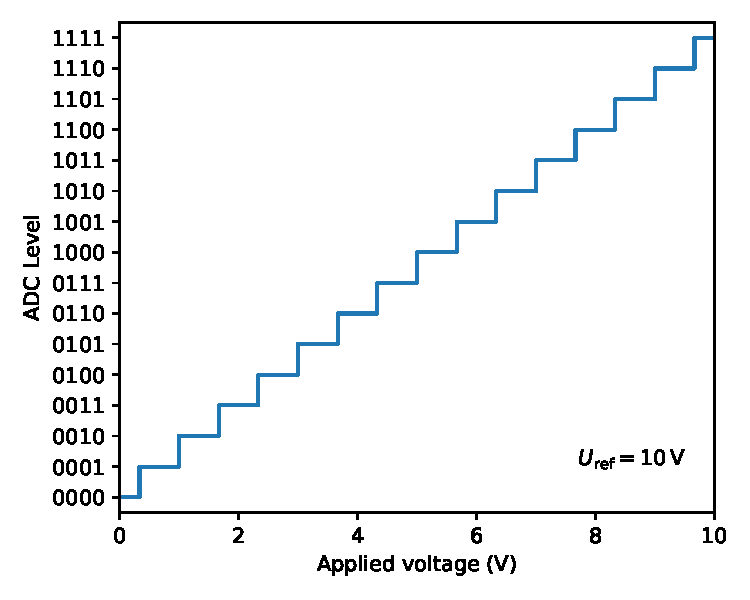
\includegraphics[width=0.625\textwidth]{graphics/00_introduction/adc.pdf}
    \caption{A 4\,bit \ac{adc} with given levels. The reference voltage is 10\,V.}
    \label{fig:intro:adc}
\end{figure}
Figure~\ref{fig:intro:adc} shows the levels of a 4\,bit ADC in binary as a function of the voltage that would be measured. The reference voltage here is $U_\mathrm{ref} = 10\,$V. This reference voltage is the voltage that the \ac{adc} can measure at most, i.e., the voltage that it will return when the \ac{adc} level is $1111$. 

Knowing the resolution $n$ of an \ac{adc}, we can easily calculate the minimum voltage difference that can be determined as 
\begin{equation}
    \Delta U = \frac{U_\mathrm{ref}}{n}.
\end{equation}
For the given example above in Figure~\ref{fig:intro:adc}, the minimum voltage would thus be $\Delta U  = 0.625\,$V. Anything smaller voltage difference requires a higher resolution \ac{adc}.


\subsection{Digital-to-Analog Conversion}\label{sec:intro:dac}

Of course, we sometimes require the opposite of an \ac{adc} and need to convert digital signal into the analog world. The device that allows for this transformation is a \ac{dac}. A true \ac{dac} takes a digital signal and returns an analog voltage by dividing a reference voltage as many times as necessary. The same resolution limitations as for an \ac{adc} also apply to a \ac{dac}. For example, a 4\,bit \ac{dac} with a reference voltage of $10\,$V can only increase the analog output in steps of 0.625\,V.

\paragraph{\Ac{pwm}} An interesting way to have a pseudo \ac{dac} is to use a process called \acf{pwm}. 
\begin{figure}[tb]
    \centering
    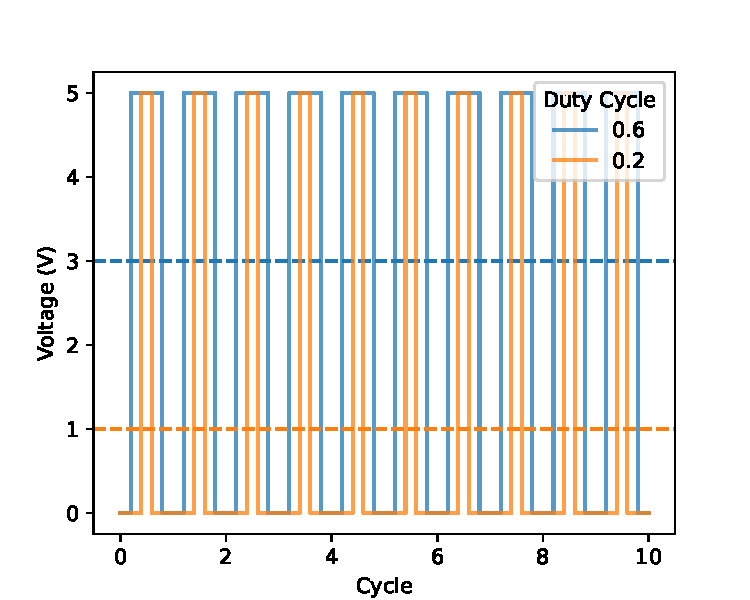
\includegraphics[width=0.625\textwidth]{graphics/00_introduction/pwm.pdf}
    \caption{\Ac{pwm} cycles and average voltage for two different duty cycles.}
    \label{fig:intro:pwm}
\end{figure}
Figure~\ref{fig:intro:pwm} shows a schematic of this process for a 5\,V pin. The digital pin is rapidly turned on and off. If it is at 5\,V for 50\% of the time, a 50\% duty cycle, the effective, smoothed-out voltage that can be seen by a ``slow'' component would be 2.5\,V. Depending on the duty cycle, a pseudo-analog output can therefore be created. A great example to use \ac{pwm} is to have a dimmable \ac{led}. \acp{led} generally have only two states, on and off, i.e., is the voltage is high enough to light them, they are bright and otherwise dark. Using \ac{pwm} however, we can turn an \ac{led} on and off in rapid succession such that it looks to the human eye as if the light source itself was dimmed.

\morebox{Analog output with \ac{pwm}}{Can you come up with a way to create a smooth analog output from a \ac{pwm} pin? Think about how your cellphone charger turns \ac{ac} into \ac{dc}.}

\section{Arduino}

For this class, we will be using an Arduino Micro. You can find more information and various alternative Arduino boards for all kinds of projects on the \href{https://www.arduino.cc}{Arduino website}.

In Appendix~\ref{app:pinout}, a schematic of the Arduino Micro board is given. This pinout diagram specifies what all the various pins on the board mean and what they are used for. It is a very handy reference for when you develop your project.

\subsection{Programming an Arduino}

The easiest way to program an Arduino is by using the \ac{ide} for Arduino that can be found \href{https://www.arduino.cc/en/software}{here}. The website also has installation guides on how to install the IDE and Arduino driver on your computer, depending on your operating system. Please see this documentation or look at it at least briefly, since it will help you with troubleshooting in case your computer does not find the Arduino board.

\paragraph{The Arduino \ac{ide}} is very useful when you are starting to learn how to program your Arduino. Under ``File'', ``Examples'' you can find eleven categories that give you many well-explained example snippets of code for various applications. We will make a lot of use of these examples, especially during the first few chapters of this workshop. The \ac{ide} also allows you to verify your code, i.e., check if it contains any errors (check button in the toolbar) and to upload your code to the Arduino itself (right arrow button in the toolbar). In order to upload your code to the Arduino board, make sure that you have the correct board selected. Go to ``Tools'', ``Board'' to select ``Arduino Micro''. Furthermore, you need to select the port on which your board is connected to the computer. To do so, go to ``Tools'', ``Port'' to select the correct one. Now you are ready to begin uploading example code or your own code.

\paragraph{Programming language overview} To program your Arduino, the code must be written in \cpp. There are many great introductions online that can help you to get started, see also the background information box below. Therefore, we will only discuss very briefly the most important rules here. These will help you to avoid the most common mistakes.

\begin{itemize}
    \item Commands and instructions are case sensitive
    \item Variables must be declared. If you need an integer for example and assign it the value three, you can do this by declaring the variable as \lstinline{int myVar = 3;}
    \item All command lines must be terminated by a semi colon \lstinline{;}
    \item Functions, loops, etc. get surrounded by curly brackets
    \item It is up to the user to make the code look readable. If you want, you can write everything into one line since line endings and function endings are defined by the above stated rules.
    \item Line comments are preceeded with \lstinline{//} while block comments use the following structure:
    \begin{lstlisting}
/*
    My comments in a block...
*/
    \end{lstlisting}
\end{itemize}

In general, the minimum file structure for your Arduino code should look similar to the following.
\begin{lstlisting}
// variable declarations, load libraries

void setup() {
  // setup code
}

void loop() {
  // main code that repeats
}
\end{lstlisting}
On the very top of your code, put variable declaration and initialization if required and load the necessary libraries. The \lstinline{setup} function is the part that runs once when you boot up your Arduino. The \lstinline{loop} function will then run repeatedly and, ideally, until you unplug or reset the Arduino. We will see later how to fill these standard functions. In addition, you can of course write your own functions with any names of your choosing, just make sure they do not collide in naming with these default functions. 

\paragraph{Debugging} When code does not do the thing we expect it to, it is often difficult to exactly see why it does not work. While the Arduino \ac{ide} catches many bugs, it cannot catch logic errors. If you simply code a script on your computer, you might debug it by printing out values to the screen. The same can be done with the Arduino. Unless you have a screen connected to the Arduino, you have to send the values to print via the serial connection to your computer for displaying. The statement \lstinline{Serial.begin(9600);} should go into your setup routine. This begins the serial communication to your computer with a \href{https://en.wikipedia.org/wiki/Baud}{baud rate} of 9600. Inside your main loop, you can then use the following print statements to write to your computer:
\begin{itemize}
    \item \lstinline{Serial.print("Hello ");} prints "Hello " without a line break.
    \item \lstinline{Serial.println("World!");} prints "World!" on the same line as the print before and then starts a new line.
\end{itemize}
To see these printed values, click in the Arduino \ac{ide} on ``Tools'' and then select ``Serial Monitor''. Note that you can also send commands from the computer to the Arduino via Serial. More information can be found \href{https://www.arduino.cc/reference/en/language/functions/communication/serial/}{here}.

\infobox{Help with programming your Arduino}{To find further information on how to program for Arduino and get yourself started with \cpp, see the following links:
\begin{itemize}
    \item \href{https://www.als.lib.wi.us/site/wp-content/uploads/2018/05/arduino-starter-kit-manual.pdf}{Starters guide for programming for Arduino}
    \item \href{https://www.arduino.cc/reference/en/}{Programming reference specifically for Arduino}
    \item \href{https://www.arduino.cc/reference/en/libraries/}{Libraries in Arduino}
    \item \href{https://www.arduino.cc/glossary/en/}{Glossary of commonly used terms}
    \item \href{https://forum.arduino.cc/}{User forum}
\end{itemize}
Note that many components that we use come with detailed instructions and guides. For example, if you buy components from \href{https://adafru.it}{Adafruit}, these parts generally come with a guide for Arduino, etc.}

\paragraph{More Help}{As with so many things in life these days, more help is generally just one \href{https://www.duckduckgo.com}{search on the internet} away. There are many forums, articles, etc., on the web that discuss building electronics with Arduino. The hope is that this workshop helps you to discover the vast possibilities and gives you the right keywords to search your way through.}


\subsection{TinkerCAD}

If you want to play with a virtual Arduino, give \href{https://www.tinkercad.com/}{TinkerCAD} a try. On its website you can simulate an Arduino, add components, write code, and then run the setup like in real life. It is a great tool to plan a project and start experimenting with setups, e.g., while you are waiting for components to ship.